
%
% The PSI Programmer's Manual
%

\documentclass[12pt]{article}
% Use this if you need to include PostScript figures or such.
%\usepackage{epsfig}
\usepackage{html}
\usepackage{color}
\usepackage{epsfig}
\usepackage{listings}
\usepackage{graphicx}
\usepackage{fancyvrb}
\usepackage{xspace}
\setlength{\textheight}{9in}
\setlength{\textwidth}{6.5in}
\setlength{\hoffset}{0in}
\setlength{\voffset}{0in}
\setlength{\headheight}{0in}
\setlength{\headsep}{0in}
\setlength{\topmargin}{0in}
\setlength{\oddsidemargin}{-0.05in}
\setlength{\evensidemargin}{-0.05in}
\setlength{\marginparsep}{0in}
\setlength{\marginparwidth}{0in}
\setlength{\parsep}{0.8ex}
\setlength{\parskip}{1ex plus \fill}
\baselineskip 18pt
\renewcommand{\topfraction}{.8}
\renewcommand{\bottomfraction}{.2}

\begin{document}

%%%%%%%%%%%%%%%%%%%%%%%
% Definitions
%%%%%%%%%%%%%%%%%%%%%%%

\newcommand{\PSI}{{\tt PSI}}
\newcommand{\PSItwo}{{\tt PSI2}}
\newcommand{\PSIthree}{{\tt PSI3}}
\newcommand{\PSIfour}{{\tt PSI4}}
\newcommand{\PSIversion}{4.0.0-alpha}
\newcommand{\PSImmmversion}{4.0.0-alpha}
\newcommand{\PSIemail}{psicode@users.sourceforge.net}

%
% Psi Modules
%
\def\module#1{{\tt #1}}
\newcommand{\libmints}{\module{libmints}}
\newcommand{\PSIdriver}{\module{psi4}}
\newcommand{\PSIinput}{\module{input}}
\newcommand{\PSIcints}{\module{cints}}
\newcommand{\PSIcderiv}{\module{cints --deriv1}}
\newcommand{\PSIdetci}{\module{detci}}
\newcommand{\PSIdetcas}{\module{detcas}}
\newcommand{\PSIdetcasman}{\module{detcasman}}
\newcommand{\PSIclag}{\module{clag}}
\newcommand{\PSIccenergy}{\module{ccenergy}}
\newcommand{\PSIccsort}{\module{ccsort}}
\newcommand{\PSIpsi}{\module{psi}}
\newcommand{\PSIcscf}{\module{cscf}}
\newcommand{\PSIoptking}{\module{optking}}
\newcommand{\PSItransqt}{\module{transqt}}
\newcommand{\PSInormco}{\module{normco}}
\newcommand{\PSIintder}{\module{intder95}}
\newcommand{\PSIgeom}{\module{geom}}
\newcommand{\PSIoeprop}{\module{oeprop}}
\newcommand{\PSIstable}{\module{stable}}

%
% Psi Library
%
\def\library#1{{\tt #1}}

%
% Psi and Unix Files
%
\def\FILE#1{{\tt file#1}}
\def\file#1{{\tt #1}}
\newcommand{\chkptfile}{\file{file32}}
\newcommand{\inputdat}{\file{input.dat}}
\newcommand{\outputdat}{\file{output.dat}}
\newcommand{\fconstdat}{\file{fconst.dat}}
\newcommand{\intcodat}{\file{intco.dat}}
\newcommand{\optaux}{\file{opt.aux}}
\newcommand{\basisdat}{\file{basis.dat}}
\newcommand{\pbasisdat}{\file{pbasis.dat}}
\newcommand{\geomdat}{\file{geom.dat}}
\newcommand{\geomout}{\file{geom.out}}

%
% Psi Keywords
%
\def\keyword#1{{\tt #1}}

%
% Psi C and Fortran Language elements
%
\def\celem#1{{\tt #1}}
\def\felem#1{{\tt #1}}

%
% Unix stuff
%
\def\unixid#1{{\em #1}} % names of groups and users
\def\shellvar#1{{\tt #1}}

%
% Nice output for function description
%
% Needs 4 arguments: function declaration,
%  description, arguments, and return values
%
% Call \initfuncdesc before using \funcdesc
%
\newcommand{\initfuncdesc}
{\newlength{\lcwidth}
\settowidth{\lcwidth}{Arguments:}
\newlength{\rcwidth}
\setlength{\rcwidth}{\linewidth}
\addtolength{\rcwidth}{-1.0\lcwidth}
\addtolength{\rcwidth}{-6.0\tabcolsep}
}

\newcommand{\funcdesc}[4]{
\celem{#1} \\
#2

\begin{tabular}{lp{\rcwidth}}
Arguments: & #3\\
Returns: & #4
\end{tabular}}

% This allows us to read in a sample file, needs the listings package
\newcommand \includesource[2] {
   \definecolor{XCodeComment}{rgb}{0.0, 0.4531, 0.0}
   \definecolor{XCodeKeyword}{rgb}{0.6641, 0.0508, 0.5664}
   \definecolor{XCodeString}{rgb}{0.7656, 0.1016, 0.0859}
   \lstset{
      language={#2}, basicstyle= \slshape \scriptsize \ttfamily,
      keywordstyle= \color{XCodeKeyword}, identifierstyle= \slshape \scriptsize,
      commentstyle= \color{XCodeComment},
      stringstyle=\ttfamily \color{XCodeString},
      showstringspaces=false,
      numbers=left,
      tabsize=4,
      title=\textit{#1},
      breaklines=true,
      showspaces=false,
      showtabs=false, frame=tb, framerule=0.5mm,
      aboveskip=5mm, belowskip=5mm,
   }
   \lstinputlisting{#1}
}

\newcommand \includeinput[1]{
   \lstdefinelanguage{psi}{
           morekeywords={geometry,label,wfn,refernce,subgroup,basis,docc,
                         print,do\_tei,ri\_basis,zmat,psi, reference,
                         df-mp2},
           sensitive=false,
           morecomment=[l]{\%}
   }
   \includesource{#1}{psi}
}


% We can enter verbatim mode by simply entering text as @text@.  No more escaping funny characters!
% \DefineShortVerb{\@}
\initfuncdesc

\begin{center}
\ \\
\vspace{2.0in}
{\bf {\Large The \PSIfour\ Programmer's Manual}} \\
\vspace{0.5in} 
T. Daniel Crawford,$^a$ C. David Sherrill,$^b$ Edward F.\ Valeev,$^{a}$ \\
Justin T. Fermann,$^c$ C. Brian Kellogg,$^c$, Andrew C. Simmonett$^c$ \\
and Justin M. Turney$^c$ \\
\ \\ 
{\em $^a$Department of Chemistry, Virginia Tech, Blacksburg, Virginia 24061} \\
\vspace{0.1in}
{\em $^b$Center for Computational Molecular Science and Technology, 
\mbox{Georgia Institute of Technology,} Atlanta, Georgia 30332-0400} \\
\vspace{0.1in}
{\em $^c$Center for Computational Quantum Chemistry, \\ 
\mbox{University of Georgia,} Athens, Georgia 30602-2525} \\
\ \\
\vspace{0.3in}
\PSIfour\ Version: \PSIversion \\
Created on: \today \\
Report bugs to: \PSIemail \\
\end{center}

\thispagestyle{empty}

\newpage
\tableofcontents

\newpage

\section{Introduction}
    \subsection{introduction} \label{introduction}
    The purpose of this manual is to provide a reasonably detailed
overview of the source code and programming philosophy of \PSIfour,
such that programmers interested in contributing to the code will have
an easier task.  Section \ref{svn} gives a succint explanation of the
steps required to obtain the source code from the main repository at
Virginia Tech.  (Installation instructions are given separately in the
installation manual or in \$PSI4/INSTALL.) \ref{Style} offers advice on
appropriate programming style for \PSIfour\ code, and section \ref{Makefiles}
describes the structure of the package's \file{Makefile}s.  Section
The appendices provide important reference material,
including the currently accepted \PSIfour\ citation and format
information for some of the most important text files used by
\PSIfour\ modules.

There are many examples included in this document to provide sample input files
and source files; these can be found in ASCII form in the \PSIfour\ source
itself.  Each included file has a path, which is relative to
\$PSI4/doc/progman, as its title and this is where the unformatted file can be
found.  The examples described herein can even be compiled from the directories
in which the source files are found.

    \subsection{History} \label{history}
    %
% History of Psi
%
% Daniel Crawford, 24 January, 1996
%

The PSI suite of {\em ab initio} quantum chemistry programs is the result
of an ongoing attempt by a cadre of graduate students, postdoctoral
associates, and professors to produce code that is efficient but also
easy to extend to new theoretical methods.  Significant effort has been
devoted to the development of libraries which are robust and easy to use.
Some of the earliest contributions to what is now referred to as ``PSI''
include a direct configuration interaction (CI) program (Robert Lucchese,
1976, now at Texas A\&M), the well-known graphical unitary group CI program
(Bernie Brooks, 1977-78, now at N.I.H.), and the original integrals code
(Russ Pitzer, 1978, now at Ohio State).  From 1978-1987, the package was
know as the {\tt BERKELEY} suite, and after the Schaefer group moved to the
Center for Computational Quantum Chemistry at the University of Georgia,
the package was renamed {\tt PSI}.  Thanks primarily to the efforts of Curt
Janssen (Sandia Labs, Livermore) and Ed Seidl (LLNL), the package was
ported to UNIX systems, and substantially improved with new input formats
and a C-based I/O system.

Beginning in 1999, an extensive effort was begun to develop \PSIthree\
--- a {\tt PSI} suite with a completely new face.  As a result of this
effort, all of the legacy Fortran code was removed, and everything was
rewritten in C and C++, including new integral/derivative integral,
coupled cluster, and CI codes.  In addition, new I/O libraries have
been added, as well as an improved checkpoint file structure and greater
automation of typical tasks such as geometry optimization and frequency
analysis.  The package has the capability to determine wavefunctions,
energies, analytic gradients, and various molecular properties based on
a variety of theories, including spin-restricted, spin-unrestricted, and
restricted open-shell Hartree-Fock (RHF, UHF, and ROHF); configuration
interaction (CI) (including a variety of multireference CI's and full
CI); coupled-cluster (CC) including CC with variationaly optimized
orbitals; second-order M{\o}ller-Plesset perturbation theory (MPPT)
including explicitly correlated second-order M{\o}ller-Plesset energy
(MP2-R12); and complete-active-space self-consistent field (CASSCF)
theory.  By January 2008, all of the C code in \PSIthree\ was 
converted to C++ to enable a path toward more object-oriented design
and a single-excecutable framework that will facilitate code reuse and 
ease efforts at parallelization.  At this same time, all of the legacy I/O
routines from {\tt PSI2} were removed, greatly streamlining the
\library{libciomr.a} library.

    \subsection{License} \label{license}
    
Mention the GPL and development policies...

\section{Obtaining \PSIfour} \label{svn}
    %
% PSI Programmer's Manual
%
% SVN Revision Control Section
% (formerly CVS)
%
% TDC, February, 1996
% Modified by TDC, December 2002
% Updated from CVS to SVN, April 2007
%

The subversion control system (SVN) (\htmladdnormallink{{\tt
    subversion.tigris.org}}{http://subversion.tigris.org/}) provides a
convenient means by which programmers may obtain the latest (or any
previous) version of the \PSIfour\ source from the main repository or
a branch version, add new code to the source tree or modify existing
\PSIfour\ modules, and then make changes and additions available to
other programmers by checking the modifications back into the main
repository.  SVN also provides a ``safety net'' in that any erroneous
modifications to the code may be easily removed once they have been
identified.  This section describes how to use SVN to access and
modify the \PSIfour\ source code.  (Note that compilation and
installation instructions are given in a separate document.)

The main repository for the \PSIfour\ Source code is currently
maintained by the Crawford group at Virginia Tech.  To check out the
code, one must first obtain an SVN account by emailing
\htmladdnormallink{{\tt crawdad@vt.edu}}{mailto:crawdad@vt.edu}.
After you have a login-id and password, you are now ready to access
the repository via a secure, SSL-based WebDAV connection, but first
you must decide which version of the code you need.

The \PSIfour\ SVN repository contains three top-level directories:
\begin{itemize}
\item {\tt trunk}: The main development area.
\item {\tt branches}: Release branches and private development
  branches are stored here.
\item {\tt tags:} Snapshots of the repository corresponding to public
  releases are stored here and should {\em never} be modified.
\end{itemize}
If you have a PSI4 SVN account, you can peruse these directories if
you like by pointing web browser to:

\noindent
{\tt https://sirius.chem.vt.edu/svn/psi4/}

\subsection{\PSIfour\ SVN Policies: Which Branch Should I Use?}
\label{section:branches}

The \PSIfour\ repository comprises a main trunk and several
release branches.  The branch you should use depends on the sort of 
work you plan for the codes:
\begin{enumerate}
\item For any piece of code already in the most recent release, bug
  fixes (defined as anything that doesn't add functionality ---
  including documentation updates) should be made {\em only} on the
  most recent stable release branch.
\item The main trunk is reserved for development of new functionality.
  This allows us to keep new, possibly unstable code away from public
  access until the code is ready.
\item Code that you do not want to put into next major release of
  \PSIfour\ should be put onto a separate branch off the main
  trunk. You will be solely responsible for maintenance of the new
  branch, so you should read the SVN manual before attempting this.
\end{enumerate}

\noindent Fig.~\ref{Fig:svn} provides a schematic of the SVN revision-control
structure and branch labeling.  Two release branches are shown, the current
stable branch, named {\tt psi-3-4}, and a planned future release, to be named
{\tt psi-3-5}.  The tags on the branches indicate release shapshots, where
bugs have been fixed and the code has been or will be exported for public
distribution.  The dotted lines in the figure indicate merge points: just
prior to each public release, changes made to the code on the stable release
branch will be merged into the main trunk.

\begin{figure}[h]
\begin{center}
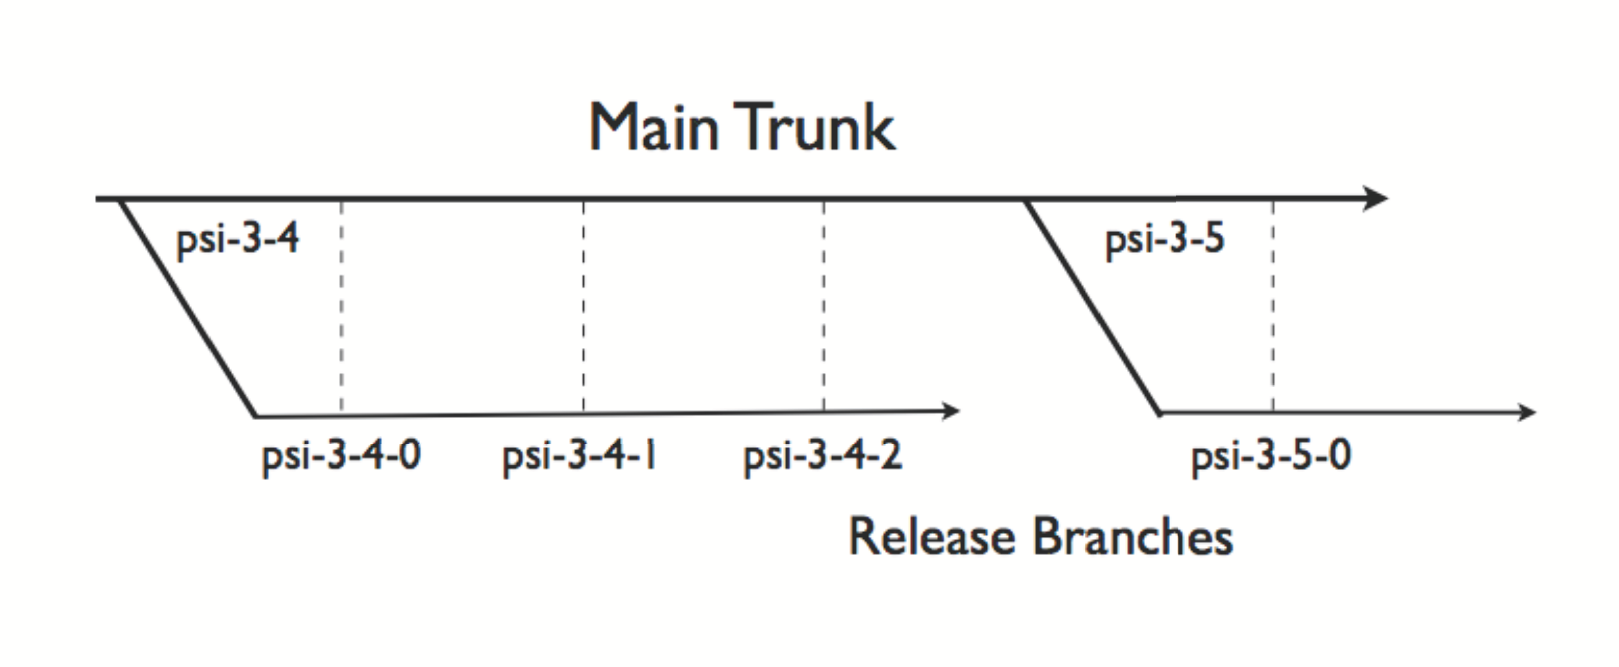
\epsfig{file=svn/svn.eps,height=6.5cm}
\end{center}
\caption{\PSIfour\ SVN branch structure with examples of branch- and
release-tag labelling.}
\label{Fig:svn}
\end{figure}

\noindent A frequently encountered problem is what to do about bug fixes
that are necessary for uninterrupted code development of the code on the
main trunk. As Rule 1 of the above policy states, all bug fixes of the code
already in the recent stable release must go on the corresponding branch,
not on the main trunk. The next step depends on the severity of the bug:
\begin{enumerate}
\item If the bug fix is critical and potentially affects every
  developer of the code on the main trunk, then \PSIfour\
  administrators should be notified of the fix. If deemed necessary,
  appropriate steps to create a new patch release will be made. Once
  the next patch release is created then the bug fixes will be merged
  onto the main trunk.  If the bug fix doesn't warrant an immediate
  new patch release, then you can incorporate the bug fix into your
  local copy of the main trunk code manually or using SVN merge
  features. This will allow you to continue development until next
  patch release is created and the bug fix is incorporated into the
  main trunk code in the repository. However you should {\em never}
  merge such changes into the main trunk yourself.
\item If the bug fix is not critical (e.g. a documentation
  update/fix), then you should wait until next patch release when it
  will be merged into the main trunk automatically.
\end{enumerate}

\noindent
The following are some of the most commonly used SVN commands for checking
out and updating working copies of the \PSIfour\ source code.

\noindent
$\bullet$ To checkout a working copy of the head of the main trunk:

{\tt svn co https://sirius.chem.vt.edu/svn/psi4/trunk/ psi4} 

\noindent
$\bullet$ To check out a working copy of the head of a specific release branch,
e.g., the branch labelled {\tt psi-4-0}:

{\tt svn co https://sirius.chem.vt.edu/svn/PSI4/branches/psi-4-0 psi4}

\noindent Note that subsequent {\tt svn update} commands in this
working copy will provide updates only on the chosen branch.  Note
also that after you have checked out a fresh working copy of the code
you must run the {\tt autoconf} command to generate a {\tt configure}
script for building the code.  (See the installation manual for
configuration, compilation, and testing instructions.)

\noindent For each of the above commands, the working copy of your
code will be placed in the directory \file{psi4}, regardless of your
choice of branch.  In this manual, we will refer to this directory
from now on as {\tt \$PSI4}.  Subsequent SVN commands are usually run
within this top-level directory.

\noindent
$\bullet$ To update your current working copy to include the latest revisions:

{\tt svn update}

\noindent
Notes: (a) This will update only the revisions on your current branch;
(b) The old {\tt -d} and {\tt -P} flags required by CVS are not necessary with SVN. 

\noindent
$\bullet$ To convert your working copy to the head of a specific branch:

{\tt svn switch https://sirius.chem.vt.edu/svn/PSI4/branches/psi-4-0}

\noindent
$\bullet$ To convert your working copy to the head of the main trunk:

{\tt svn switch https://sirius.chem.vt.edu/svn/psi4/trunk/}

\noindent
$\bullet$ To find out what branch your working copy is on, run this in your
top-level \PSIfour\ source directory:

{\tt svn info | grep URL}

\noindent
This will return the SVN directory from which your working copy was
taken, e.g.,

\noindent
{\tt URL: https://sirius.chem.vt.edu/svn/PSI4/branches/psi-4-0}

\noindent
Some words of advice:
\begin{enumerate}
\item Most SVN commands are reasonably safe, 

\item Unlike CVS, you shouldn't use {\tt svn update} to see the status
  of your working copy.  With SVN you should use {\tt svn status} to
  see if you've modified any files or directories.  If you want a
  direct comparison with the repository, you should use {\tt svn status -u}.
\item Read the SVN manual.  Seriously.
\begin{center}
\htmladdnormallink{{\tt
http://svnbook.red-bean.com/}}{http://svnbook.red-bean.com/}
\end{center}
\item If you're about to start some significant development or bug-fixes,
first update your working copy to the latest version on your branch.
In addition, if you do development over a long period of time (say weeks to
months) on a specific module or modules, be sure to run a {\tt svn status -u}
occasionally. In can be {\em very} frustrating to try to check in lots
of changes, only to find out that the \PSIfour\ has changed dramatically
since your last update.
\end{enumerate}

\subsection{Checking in altered \PSIfour\ binaries or libraries}

If you have changes to Psi binaries or libraries which already exist, one
of two series of steps is necessary to check these changes in to the main
repository. The first series may be followed if all changes have been made
only to files which already exist in the current version. The second series
should be followed if new files must be added to the code in the repository.

\begin{itemize}
\item No new files need to be added to the repository. We will use
\library{libciomr} as an example. 
\begin{enumerate}
\item {\tt cd \$PSI4/src/lib/libciomr}
\item {\tt svn ci -m ``Put comments here.''}
\end{enumerate}
\item New files must be added to the repository. Again, we use 
\library{libciomr}
as an example. Suppose the new file is named \file{great\_code.cc} .
\begin{enumerate}
\item {\tt cd \$PSI4/src/lib/libciomr} 
\item {\tt svn add great\_code.cc} 
\item {\tt svn ci -m ``Put comments here.''}
\end{enumerate}
\end{itemize}

The \file{svn ci} command in both of these sequences will examine all
of the code in the current \file{libciomr} directory against the
current version of the code in the main repository. Any files which
have been altered (and for which no conflicts with newer versions
exist!) will be identified and checked in to the main repository (as
well as the new file in the second situation).

SVN requires that you include a comment on your changes.  However,
unlike CVS, SVN prefers that you put your comments on the command-line
rather than editing a text file.  I prefer the CVS way, but this is a
minor pain compared to all the advantages of SVN, in my opinion.

\subsection{Adding entirely new code to the main \PSIfour\ repository} 
\label{checkin_new}

If the programmer is adding a new executable module or library to the
\PSIfour\ repository, a number of important conventions should be followed:

\begin{enumerate}
\item Since such changes almost always involve additional functionality,
new modules or libraries should be added only on the main SVN trunk.
See section \ref{section:branches} for additional information.

\item The directory containing the new code should be given a name
  that matches the name of the installed code (e.g. if the code will
  be installed as \module{newcode}, the directory containing the code
  should be named \file{newcode}). New executable modules must be
  placed in \shellvar{\$PSI4}\file{/src/bin} and libraries in
  \shellvar{\$PSI4}\file{/src/lib} of the user's working copy.

\item The Makefile should be converted to an input file for the
  configure script (\file{Makefile.in} --- see any of the current
  \PSIfour\ binaries for an example) and should follow the
  conventions set up in all of the current \PSIfour\
  \file{Makefiles}. This includes use of \file{MakeVars} and
  \file{MakeRules}.

\item New binaries should be added to the list contained in
  \shellvar{\$PSI4}\file{/src/bin/Makefile.in} so that they will be
  compiled automatically when a full compilation of the \PSIfour\
  distribution occurs. This step is included in the sequence below.

\item A documentation page should be included with the new code (see
  section \ref{Documentation} for more information). As a general
  rule, if the code is not ready to have a documentation page, it is
  not ready to be installed in \PSIfour.

\item The \file{configure.ac} file must be altered so that users may
  check out copies of the new code and so that the \file{configure}
  script will know to create the Makefile for the new code. These
  steps are included in the sequence below.

\end{enumerate}

Assume the new code is an executable module and is named
\module{great\_code}. The directory containing the new code must
contain only those files which are to be checked in to the repository!
Then the following steps will check in a new piece of code to the main
repository:

\begin{enumerate}
\item {\tt cd \$PSI4/src/bin}
\item {\tt svn add great\_code}
\item {\tt svn ci -m ``Put comments here.''}
\item {\tt cd \$PSI4}
\item Edit \file{configure.ac} and add \file{great\_code} to the list. 
\item {\tt svn ci configure.ac -m ``Put comments here.''}
\item {\tt autoconf} 
\item {\tt cd \$PSI4/src/bin} 
\item Edit \file{Makefile.in} and add \file{great\_code} to the list. 
\item {\tt svn ci Makefile.in -m ``Put comments here.''}
\end{enumerate}
At this point, all of the code has been properly checked in, but you
should also test to make sure that the code can be checked out by
other programmers, and that it will compile correctly. The following
steps will store your personal version of the code, check out the new
code, and test-compile it:
\begin{enumerate}
\item {\tt cd \$PSI4/src/bin}
\item {\tt mv great\_code great\_code.bak}
\item {\tt cd \$PSI4/..}
\item {\tt svn update}
\item {\tt cd \$objdir}
\item {\tt \$PSI4/configure -}{\tt -prefix=\$prefix}
\item {\tt cd src/bin/great\_code}
\item {\tt make install}
\end{enumerate}
(Note that \$prefix and \$objdir to the installation and compilation
 directories defined in the \PSIfour\ installation instructions.)
Your original version of the code remains under \file{great\_code.bak},
but should be no longer necessary if the above steps work. Note that it is
necessary to re-run \file{configure} explicitly, instead of just running
\file{config.status}, because the latter contains no information about
the new code.

\subsection{Updating checked out code}

If the code in the main repository has been altered, other users' working
copies will of course not automatically be updated.  In general, it is
only necessary to execute the following steps in order to completely update
your working copy of the code:

\begin{enumerate}
\item {\tt cd \$PSI4}
\item {\tt svn update}
\end{enumerate}

This will examine each entry in your working copy and compare it to
the most recent version in the main repository. When the file in the
main repository is more recent, your version of the code will be
updated. If you have made changes to your version, but the version in
the main repository has not changed, the altered code will be
identified to you with an ``M''. If you have made changes to your
version of the code, and one or more newer versions have been updated
in the main repository, SVN will examine the two versions and attempt
to merge them -- this process often reveals conflicts, however, and is
sometimes unsuccessful. You will be notified of any conflicts that
arise (labelled with a ``C'') and you must resolve them manually.

If new directories have been added to the repository, the update above
will automatically add them to your working copy.  However, you may
need to re-run {\tt autoconf} and configure ({\tt
  \$objdir/config.status --recheck} is a convenient command) to be
able to build the new code.

\subsection{Removing code from the repository}
If alterations of libraries or binaries under Psi involves the deletion of 
source code files from the code, these must be explicitly removed through SVN.

The following steps will remove a source code file named \file{bad\_code.F} 
from a binary module named \module{great\_code}:
\begin{enumerate}
\item {\tt cd \$PSI4/src/bin/great\_code}
\item {\tt svn remove bad\_code.F}
\item {\tt svn ci -m ``Put comments here.''}
\end{enumerate}

\subsection{Checking out older versions of the code}
It is sometimes necessary to check out older versions of a piece of code.
Assume we wish to check out an old version of \PSIdetci. If this
is the case, the following steps will do this:
\begin{enumerate}
\item {\tt cd \$PSI4/src/bin/detci}
\item {\tt svn co --revision \{2002-02-17\}}
\end{enumerate}

This will check the main repository and provide you with the code as
it stood exactly on February 17th, 2002. 

\subsection{Examining the revision history}
It can be very useful to use cvs to see what recent changes have been
made to the code.  Anytime one checks in a new version of a file, SVN
requires the user to provide comments on the changes with the {\tt -m}
flag.  These comments go into a log information that may be easily
accessed through SVN.  To see what changes have been made recently to
the file \file{detci.cc}, one would go into the \file{detci} source
directory and type
\begin{verbatim}
svn log detci.cc
\end{verbatim}
Checking the log files is a very useful way to see what recent changes might 
be causing new problems with the code.

\subsection{The structure of the \PSIfour\ Source Tree}
\label{psitree} 

Your working copy of the \PSIfour\ source code includes a number of
important subdirectories:

\begin{itemize}
\item \shellvar{\$PSI4}\file{/lib} -- Source files for
  OS-independent ``library'' data.  This includes the main basis set
  data file (\file{pbasis.dat}) and the \PSIfour\ program execution
  control file (\file{psi.dat}), among others.  These files are
  installed in \file{\$prefix/share}.

\item \shellvar{\$PSI4}\file{/include} -- Source files for
  OS-independent header files, including \file{physconst.h} (whose
  contents should be obvious from its name), \file{psifiles.h}, and
  \file{ccfiles.h}, among others.  These files are installed in
  \$prefix/include.

\item \shellvar{\$PSI4}\file{/src/util} -- Source code for the utility
  program \module{tocprint}.  (Note that the \module{tmpl} module is
  no longer used and will eventually disappear.)

\item \shellvar{\$PSI4}\file{/src/lib} -- Source code for the
  libraries, including \library{libpsio}, \library{libipv1},
  \library{libchkpt}, etc.  The include files from the library
  source are used directly during the compilation of PSI to 
  avoid problems associated with incomplete installations.  Some
  include files are architecture-dependent and go in an include
  subdirectory of the compilation (object) directory.

\item \shellvar{\$PSI4}\file{/src/bin} -- Source code for the
  executable modules.
\end{itemize}

After compilation and installation, the \file{\$prefix} directory
contains the executable codes and other necessary files.  {\bf NB:}
The files in this area should never be directly modified; rather, the
working copy should be modified and the \PSIfour\ \file{Makefile}
hierarchy should handle installation of any changes.  The structure of
the installation area is:

\begin{itemize}
\item \file{\$prefix/bin} -- The main executable directory.  This
  directory must be in your path in order for the driver program,
  \module{PSI4}, to find the modules.

\item \file{\$prefix/lib} -- The \PSIfour\ code libraries.  (NB: The
  description of \PSIfour\ \file{Makefiles} later in this manual will
  explain how to use the libraries.)

\item \file{\$prefix/include} -- Header files.  These are not actually
  used during the compilation of PSI but are useful for inclusion by
  external programs because they are all in the same directory.

\item \file{\$prefix/share} -- OS-independent data files, including
  basis set information.  (Do not edit this file directly; any changes
  you make can be overwritten by subsequent {\tt make} commands.)

\item \file{\$prefix/doc} -- \PSIfour\ documentation, including
  installation, programmer, and user manuals.
\end{itemize}


\section{Python and \PSIfour} \label{python}
    One of the most significant changes introduced in version 4 was the use of
Python.  The input file is actually a Python script, which interacts with a Psi
Python module to perform computations.  In order for this to happen, the C++
binding must be known to Python; this is all done in the 
{\tt \$PSI4/src/bin/psi4/python.cc} file.  For example, we have an SCF module, with
the C++ signature
{\tt PsiReturnType cscf::cscf(Options \&options);}
To allow Python to use this, we first define a little wrapper function
\begin{verbatim}
double py_psi_scf()
{
    if (scf::scf(Process::environment.options) == Success)
        return Process::environment.globals["CURRENT ENERGY"];
    else
        return 0.0;
}
\end{verbatim}
This does a couple of things to automate things a) it passes the default
options object into SCF automatically, so that the user doesn't have to, and b)
checks the return value, and will return the energy, which is posted to the
globals map, back to Python.  Note that this is C++ code, within \PSIfour\ so
it is aware of all global objects, such as PSIO, Chkpt and Options.  Now we
have this simple function call, we can tell Python about it:
\begin{verbatim}
def("scf",  py_psi_scf);
\end{verbatim}
This binds the keyword ``scf'' to the newly created wrapper function, allowing
the user to type ``scf()'' in their Python input file to fire up the SCF
module.  Similarly, the user might want to be able to call {\tt Molecule}'s
member functions directly from Python.  This can also be done easily:

\begin{verbatim}
class_<Molecule, shared_ptr<Molecule> >("Molecule").
        def("print_to_output", &Molecule::print).
        def("nuclear_repulsion_energy", &Molecule::nuclear_repulsion_energy);
\end{verbatim}

This first defines the keyword {\tt Molecule} to refer to the C++ {\tt
Molecule}; the {\tt shared\_ptr<Molecule>} keyword tells Python to store it as
a shared pointer, which ensures that the object will not be deleted until both
C++ and Python have no more references to it.  The member functions to be bound
are then specified by a chained sequence of {\tt def} calls (note the periods),
terminated by a semicolon.  Then, if the user had defined a molecule called
``water'', they could print its geometry simply with the command {\tt
water.print\_to\_output()}.

Direct interaction with the Psi module from Python requires function calls that
look like {\tt psi4.call\_some\_function()}.  This is not very friendly to
your average user, so a preprocessor checks for known Psi syntax and turns it
into valid Python, before handing it off for excecution.  This preprocessor is
purely Python, and lives in {\tt \$PSI4/lib/python/input.py}.  For example, the
following text \begin{verbatim}
set scf {
    SCF_TYPE DIRECT
    BASIS cc-pVDZ
    RI_BASIS_SCF cc-pVDZ-HF
    guess core
}
\end{verbatim}
is converted to the following text
\begin{verbatim}
psi4.set_default_options_for_module("SCF")
psi4.set_option("SCF_TYPE", "DIRECT")
psi4.set_option("BASIS", "cc-pVDZ")
psi4.set_option("RI_BASIS_SCF", "cc-pVDZ-HF")
psi4.set_option("GUESS", "core")
\end{verbatim}
which can be handled by Python.

There are a number of other utilities, which are entirely Python, located in
{\tt \$PSI4/lib/python}.  These provide convenient functions to the user, such
as {\tt table}.


\section{Testing} \label{testing}
    The \PSIfour\ test suite is designed to maximize code reuse and
provide testing in \$prefix before the \PSIfour\
executables have been installed. The configure script in \$PSI4 
will take all the necessary files in \$PSI4/tests
with the .in stub: Makefile.in, MakeRules.in, MakeVars.in,
and runtest.pl.in, replace variables with system specific parameters,
and copy/create the testing files and directories in \$prefix/tests.
The tests should be run in the object directory before installation.

If you have just added a new module for performing, say multireference 
coupled cluster, and you would like to add a test case to the current 
test suite, here is what you should do.  
\begin{enumerate}
\item Copy one of the existing test case directories to an 
      appropriately named directory for the new test case.

\item Create an appropriate input file for running the new module. 
      Then, if your program produced the correct data, rename
      the output files to *.ref. Follow the convention of the 
      existing test cases.

\item If the test case is small, add the directory name to the list
      in \$PSI4/tests/Makefile.in.  If the test is particularly tricky,
      see the psi\_start or rhf-stab test cases as an example.

\item All the testing functionality is located in the perl library
      \file{runtest.pl.in}. If you are testing for a quantity that
      is not searched for currently, then add a function to the 
      library following the format of the functions already available.
      If you have added functionality to the \PSIfour\ driver,
      make sure to update the appropriate functions in \file{runtest.pl.in}.

\item Add the location of the Makefile for the new test case
      to the configure script in \$PSI4.

\end{enumerate}

Please contact one of the authors of \PSIfour\ before making any
major changes or if you have a problem adding a new test case.
Remember, if all else fails, read the source code.


\section{Sample Codes} \label{sample-codes}
    In this chapter we demonstrate how to write code for \PSIfour\ using some simple
examples.  It can be quite daunting to develop code in an unfamiliar programming
environment, so a good starting point is to write code that requires little
knowledge of the existing code structure.  In this regard, the modular nature
of \PSIthree\ made it a perfect development platform, with each ``module''
existing as a standalone code.  With the transition to a single executable
paradigm in \PSIfour, developing new code is still a simple process; in fact
the availability of library functions to perform most tasks makes it even
easier to get started with programming in \PSIfour, as we will demonstrate.

    \subsection{Integrals} \label{integrals}
    As noted previously, we want to start from a code that's not too tightly
integrated with the \PSIfour\ code itself, so we beginwith a Makefile that will
allow us to write a standalone code that includes all requisite \PSI\
libraries.  We're going to write a small sample code that generates integrals,
which involves two just two source files.  We begin by defining a Makefile that
will include all of the \PSIfour\ libraries and header files, so that we can
take full advantage of the wide range of features implemented without having to
worry about the details of their implementation.
\newpage
\includesource{sample-codes/integrals/Makefile}{make}
Only a few lines of this makefile need to be modified to utilize it for other
programming projects; we'll concentrate on them.  On the second line, we define
the name of the executable to be generated, in this example we opt for the
unimaginative title of {\tt integrals}.  Line 4 provides the list of source files
that the project comprises; these will be detailed below.  The top source
directory for the \PSIfour\ installation and the top object directory (where
\PSIfour\ was compiled) should be provided on lines 6 and 8, respectively.
Lines 10 and 11 describe the flags needed to link in the {\tt BLAS} and {\tt
LAPACK} libraries and might need a combination of ``-Lfolder\_name'' and
``-llibrary\_name'', depending on your system's setup.  Finally, the compiler
and flags are detailed on lines 12--17.  It's a good idea to use the flags
described on line 16 for development; they speed up code compilation and
provide lots of information for standard debugging tools.  As noted in the
Makefile itself, nothing below line 17 should require modification for any
\PSIfour\ project.

The \PSIfour\ driver program provides a lot of functionality that we forgo in
writing a standalone code; this is instead emulated in the {\tt main.cc} file,
shown below.  
\includesource{sample-codes/integrals/main.cc}{C++}

All modules in \PSIfour\ must have the argument list and return type shown on
line 13.  The possible return types, defined by an enumeratable constant are
documented in {\tt psi4-dec.h}.  Notice that all of the code must live in it's
own namespace within the {\tt psi} namespace, in this case it's in the {\tt
psi::integrals} namespace.  Without this nesting, functions belonging to
different parts of the code, but having the same name, would cause conflicts.
The {\tt read\_options} function is responsible for setting up the {\tt
Options} object, which contains the list of user-provided options.  Lines
25--32 are important - these provide the list of keywords expected by the code,
their types, and their default values (if any).  This part of the code will be
inserted into the \PSIfour\ driver when the module is ready for merging with
the \PSIfour\ distribution; this process will be detailed later in the chapter.
Notice the special formats of the comments on lines 27 and 30.  These are still
valid {\tt C++} comments, but the extra hyphens inside are essential in this
context.  Whenever adding any options for any module, you must comment them as
shown - this will ensure that the keywords are automatically inserted into the
\PSIfour\ users' manual.  The {\tt main} function does a little setting up of
the \PSI\ input and output environments, before calling the module code we're
developing (on line 53) and shutting down the \PSIfour\ I/O systems.

The module we're developing is in the following source file.
\includesource{sample-codes/integrals/integrals.cc}{C++}

Given the extensive documentation within the code, we'll not describe this file
line-by-line; however, some points warrant elaboration.  Notice that the entire
module is encapsulated in the {\tt psi::integrals} namespace (lines 6 and 92).
This simple exmple has only one function body, which lives in a single source
file - if more functions and/or source files were added, these too would have
to live in the {\tt psi::integrals} namespace.  On lines 29 and 31 of {\tt
main.cc} we told the parser which keywords to expect, and provided default
values in case the user omited them from the input.  This makes retrieving
these options very clean and simple ({\it c.f.} lines 11 and 12 of {\tt
integrals.cc}).  Each \PSIfour\ module will have to initialize its own local
{\tt PSIO} and {\tt Chkpt} objects to perform I/O and to retrieve information
from previously run modules.  Notice that these objects are created within
smart pointers (see section XXX for more information) so that they are
automatically deleted when they go out of scope, thus reducing the burden on
the programmer.  Likewise, the basis sets, matrices and integral objects are
allocated using smart pointers.



    \subsection{MP2 With Density Fitting} \label{df-mp2}
    Here's a more realistic example of a \PSIfour\ module - a reasonably efficient
DF-MP2 code.  The major advantage of density fitting methods is the replacement
of four-index integrals with products of three-index integrals.  With the
\libmints\ class, \PSIfour\ can compute these integrals easily and efficiently,
as we will now demonstrate.  The Makefile for this project is

\includesource{sample-codes/df-mp2/Makefile}{make}

As with the integral code in section \ref{integrals}, we make a simple
\module{main} routine to set up the \PSI\ I/O routines and call our new module.
Notice that the hyphens are absent from the namespace definition, as they are
not allowed in C++, although underscores are valid.

\includesource{sample-codes/df-mp2/main.cc}{C++}

The code for the Module itself is a little more complex than before, and a few
extra features are used that were absent from the \module{integrals} code.  On
lines 31 and 36, instead of throwing a generic \module{PsiException} we throw a
more specific \module{InputException}.  The full list of exceptions available
can be found on in the \module{Doxygen} documentation or in the
\file{exceptions.h} file, which is in \$PSI4/include.  The default scale
factors are defined in \file{main.cc}, where the options are declared and not
where the options are read in on lines 51 and 52.

This code shows off the fledibility of the \libmints\ module, which can accept
arbitrary basis sets for each index in the four index integral.  Passing a
special {\tt zero\_basis\_set} object for one index allows us to compute
three-center integrals efficiently - see the \module{IntegralFactory} creation
on lines 174 and 175.  

\includesource{sample-codes/df-mp2/df-mp2.cc}{C++}

The formation of the metric matrix is performed in a function defined in a
seperate file.  Breaking large chunks of code into smaller, more manageable,
segments is usually a good strategy; if fact, the \file{main.cc} should
probably be further subdivided.  To do this, we need a declaration of the
external function to be defined (lines 12 and 13 of \file{df-mp2.cc}) before
defining the function itself in a seperate file, in this case we create the
following file:

\includesource{sample-codes/df-mp2/df-mp2-formJ.cc}{C++}

We also have to remember to add this new source file to the list of sources in
the \file{Makefile}, but it's as easy as that.  A sample input file that will
drive this code is shown below.

\includeinput{sample-codes/df-mp2/input.dat}

Notice how the \keyword{print} keyword is in a special {\tt DF-MP2} section of
the input file - this is to prevent the \module{input} module from parsing the
print keyword and producing excessive output when the print level is high.
This code requires \module{input}, \module{cints} and \module{cscf} to be run
before it can function.


\newpage
\appendix


\end{document}
